\documentclass{article}
\usepackage{setspace,fullpage,xcolor}
\usepackage{booktabs} % For formal tables
\usepackage{tabularx} % For adjustable-width columns
\usepackage{tikz, enumitem, xcolor}
\usetikzlibrary{matrix}


\begin{document}

\begin{center}
\textbf{Stat 346 Homework \#10}\\
\vspace{0.3in}
\end{center}

\section*{Homework Questions}

\begin{enumerate}

\item A call option has a strike price of \$60 and expires in 10 months. The profit of the call option when the spot price at expiration is \$64 is \$2.12. What is the profit of the call option if the spot price at expiration is \$56?  \textcolor{red}{[-1.88]}

\item For a 2-year put option priced with a 4 period binomial tree you are given that $P_{d^4} = 31.12$, $P_{ud^3} = 15.87$, $P_{u^2d^2} = 3.91$ and $P_{u^3d} = P_{u^4} = 0$. The risk free interest rate is $r = 0.04$ and $p = 0.7143$. What is the premium of the put option? \textcolor{red}{[2.07]}

\item Determine the price of a 1-year 22-strike European call option using Black Scholes for a stock with an initial stock price of 25 and a volatility of $\sigma = 0.10$. The risk free interest rate is $r = 0.04$. \textcolor{red}{[3.91]}

\item How would you delta hedge your position if you purchased the option in Problem 3? \textcolor{red}{[Short sell 0.958 shares of stock]}

\item Determine the price of a 3 month 40-strike European put option using Black Scholes for a stock with an initial stock price of 38 and a volatility of $\sigma = 0.15$. The risk free interest rate is $r = 0.06$. 

\item How would you delta hedge your position if you purchased the option in Problem 5?

\item The volatility for a stock is unknown and $r = 0.04$. The initial stock price is \$110. If a 108-strike 8 month call option has a premium of \$10.36 under a Black Scholes framework and it is known that $d_1 = 0.34$. What is the volatility of the stock? \textcolor{red}{[22\%]}

\item The following is a stock price tree for a particular stock using $h = 4/12$

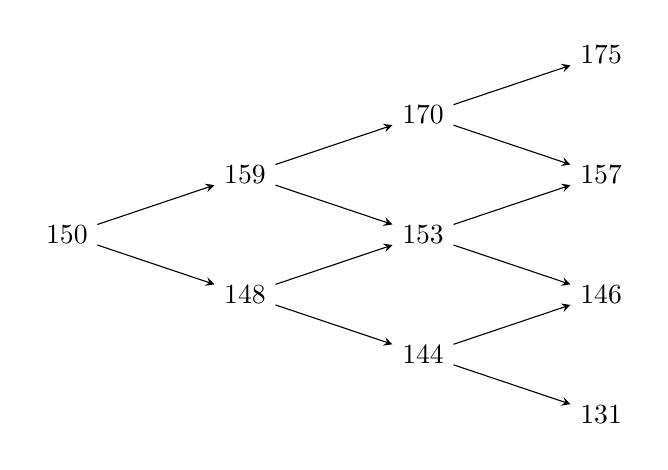
\begin{tikzpicture}[>=stealth,sloped]
    \matrix (tree) [%
      matrix of nodes,
      minimum size=.3cm,
      column sep=1.5cm,
      row sep=.3cm,ampersand replacement=\&
    ]
    {
    	\&  \&  \& 175 \\
          \&   \& 170 \& \\
          \& 159 \&  \& 157 \\
      $150$ \&   \& 153 \& \\
          \& 148 \&  \& 146  \\
          \&   \& 144  \& \\
          \&  \&  \& 131  \\
    };
    \draw[->] (tree-4-1) -- (tree-3-2) node [midway,above] {};
    \draw[->] (tree-4-1) -- (tree-5-2) node [midway,below] {};
    \draw[->] (tree-3-2) -- (tree-2-3) node [midway,above] {};
    \draw[->] (tree-3-2) -- (tree-4-3) node [midway,below] {};
    \draw[->] (tree-5-2) -- (tree-4-3) node [midway,above] {};
    \draw[->] (tree-5-2) -- (tree-6-3) node [midway,below] {};
    \draw[->] (tree-4-3) -- (tree-3-4) node [midway,above] {};
    \draw[->] (tree-2-3) -- (tree-3-4) node [midway,above] {};
    \draw[->] (tree-4-3) -- (tree-5-4) node [midway,below] {};
    \draw[->] (tree-2-3) -- (tree-1-4) node [midway,above] {};
    \draw[->] (tree-6-3) -- (tree-7-4) node [midway,below] {};
    \draw[->] (tree-6-3) -- (tree-5-4) node [midway,below] {};

  \end{tikzpicture}

The probability of moving up is $p = 0.4$. The interest rate is $r = 0.05$. Using this stock price tree, determine the price of a 1 year European call option with a strike price of 147. 

\item Suppose instead you wish to purchase an 8-month call option with strike price of 147. Using the tree in problem 8, what would the price be? 

\subsection*{Review Questions}

 

Below are the summaries for each accident, including the accident year, policy year, payments made, and case reserves by year.

\subsection*{Accident 1}
\begin{itemize}
       \item Date of Accident: June 15, 2011
        \item Policy Written: January 10, 2011
\end{itemize}
\begin{tabular}{lcc}
\toprule
Year & Payments Made (\$) & Case Reserves (\$) \\
\midrule
2011 & 5,000 & 7,000 \\
2012 & 4,500 & 3,000 \\
2013 & 2,000 & 1,500 \\
\bottomrule
\end{tabular}

\subsection*{Accident 2}
\begin{itemize}
       \item Date of Accident: March 22, 2012
        \item Policy Written: December 5, 2011
\end{itemize}
\begin{tabular}{lcc}
\toprule
Year & Payments Made (\$) & Case Reserves (\$) \\
\midrule
2012 & 4,000 & 5,000 \\
2013 & 3,000 & 3,500 \\
\bottomrule
\end{tabular}

\subsection*{Accident 3}
\begin{itemize}
        \item Date of Accident: November 8, 2012
        \item Policy Written: July 15, 2012
\end{itemize}
\begin{tabular}{lcc}
\toprule
Year & Payments Made (\$) & Case Reserves (\$) \\
\midrule
2012 & 1,500 & 2,000 \\
2013 & 2,500 & 2,000 \\
\bottomrule
\end{tabular}

\subsection*{Accident 4}
\begin{itemize}
        \item Date of Accident: July 4, 2013
        \item Policy Written: February 20, 2013
\end{itemize}
\begin{tabular}{lcc}
\toprule
Year & Payments Made (\$) & Case Reserves (\$) \\
\midrule
2013 & 4,000 & 2,000 \\
\bottomrule
\end{tabular}

\subsection*{Accident 5}
\begin{itemize}
       \item Date of Accident: December 15, 2013
        \item Policy Written: May 30, 2013
\end{itemize}
\begin{tabular}{lcc}
\toprule
Year & Payments Made (\$) & Case Reserves (\$) \\
\midrule
2013 & 3,500 & 4,500 \\
\bottomrule
\end{tabular}

\item Determine the following:
\begin{enumerate}
\item Calendar year 2013 losses \textcolor{red}{[18,500]}
\item Accident year 2012 losses as of Dec 1, 2013 \textcolor{red}{[16,500]}
\item Policy year 2011 losses as of Dec 1, 2013 \textcolor{red}{[23,500]}
\end{enumerate}

\item Construct a cumulative claims triangle for incurred losses based on only these claims. 

{\color{red}
\begin{table}[h]
\begin{tabular}{@{}lccc@{}}
\toprule
\textcolor{red}{Accident Year} & \textcolor{red}{Dev Year 0} & \textcolor{red}{Dev Year 1} & \textcolor{red}{Dev Year 2} \\ \midrule
\textcolor{red}{2011}          & \textcolor{red}{12,000}     & \textcolor{red}{12,500}     & \textcolor{red}{13,000}     \\
\textcolor{red}{2012}          & \textcolor{red}{12,500}      & \textcolor{red}{16,500}     & \textcolor{red}{-}          \\
\textcolor{red}{2013}          & \textcolor{red}{14,000}     & \textcolor{red}{-}          & \textcolor{red}{-}          \\ \bottomrule
\end{tabular}
\end{table}
}

\item Find loss development factors for this claims triangle using simple averages. \textcolor{red}{[1/0:  1.18; 2/1: 1.04]}

\item Assume a tail factor of 1.01. Determine ultimate losses for the years 2012 and 2013 using the claims triangle method. \textcolor{red}{[2012: 17160; 2013: 17192.93]}

\item Based on this results, what is IBNR for accident year 2013? \textcolor{red}{[3192.93]}

\item Based on this results, what are total reserves for accident year 2013? \textcolor{red}{[9692.93]}


\item Now assume that we have a trend for losses of $\delta = 0.02$. Based on these losses, if we were to use a weighted average of 80\% of 2013 ultimate losses and 20\% of 2012 ultimate losses, what would losses be when trended to policy year 2015?  \textcolor{red}{[18140.39]}

\item Suppose we have total fixed expenses of 100 and 4 exposure units. If the permissible loss ratio is 80\%, what would the rate be for the 2015 policy using the loss cost method? \textcolor{red}{[5700.12]}

\end{enumerate}

\end{document}
